\chapter{Équations de Maxwell}
\begin{tcolorbox}
   \begin{figure}[H] %h:当前位置, t:顶部, b:底部, p:浮动页
     \centering
     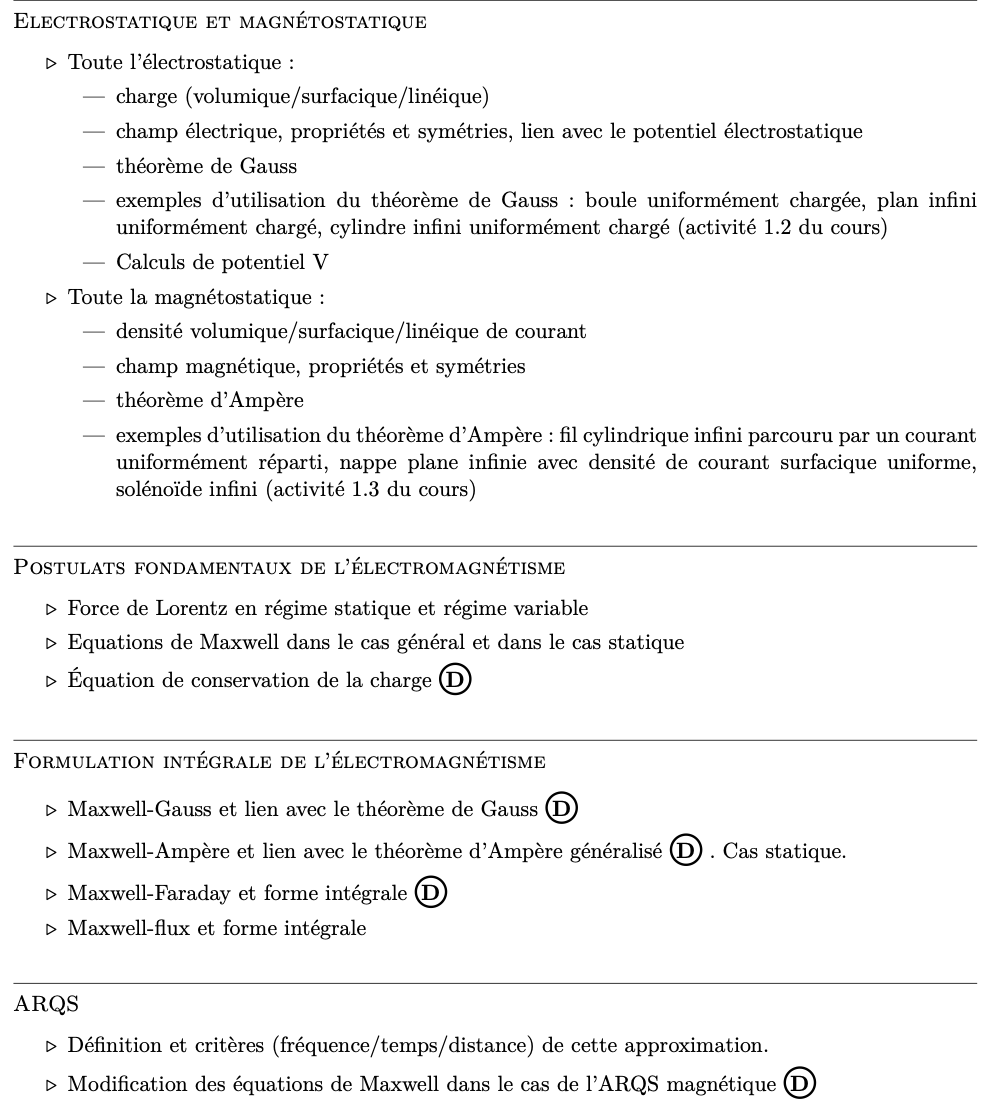
\includegraphics[width=0.9\textwidth]{./assets/Programme du chapitre 1.png}
     \caption{Programme du chapitre 1}
     \label{fig:Programme du chapitre 1}
   \end{figure}
\end{tcolorbox}

\newpage
\section{Rappels} % (fold)
\label{sec:Rappels}
Pour plus d'information, aller voir mes notes d'électromagnétisme(1re année) : \href{https://github.com/Languisher/CPGE-Notes/blob/main/Notes/Notes%20-%20Essentiels/ElectroMag.pdf}{le cours d'éléctromagnétisme}.

  \subsection{Distribution de charges} % (fold)
  \label{sub:Distribution de charges}
  
  % subsection Distribution de charges (end)
\begin{Prop}{Distribution de charges}{}

\begin{itemize}

    \item Linéique
      \[
        \mathrm{d}q(P) = \lambda(P) \times \mathrm{d}l
      \]
    \item Surfacique
      \[
        \mathrm{d}q(P ) = \sigma(P) \times \mathrm{d}\Sigma
      \]
    \item Volumnique
      \[
        \mathrm{d}q(P) = \rho(P) \times \mathrm{d}V
      \]
\end{itemize}
\end{Prop}

\subsection{Distribution de courant} % (fold)
\label{sub:Distribution de courant}

% subsection Distribution de courant (end)
\begin{Definition}[colbacktitle=red!75!black]{Vecteur densité de courant}{}
Chaque porteur de charges est en mouvement à la vitesse moyenne $\overrightarrow{v }(M,t)$. 

\begin{figure}[H] %h:当前位置, t:顶部, b:底部, p:浮动页
  \centering
  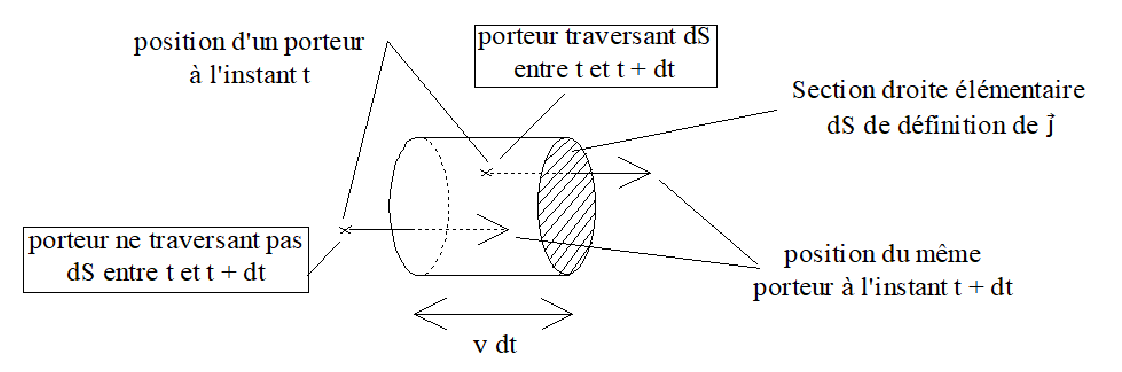
\includegraphics[width=0.8\textwidth]{./assets/Vecteur densité de courant.png}
  \caption{Vecteur densité de courant}
  \label{Vecteur densité de courant}
\end{figure}

Calculons la charge $\delta ^{2} q$ qui traverse un élément de surface $\overrightarrow{\mathrm{d}S}$ pendant une durée $\mathrm{d
}t$ :
\begin{equation}
  \rho \times (v \mathrm{d}t \times \mathrm{d}s) = \delta ^2 q 
\end{equation}.

On définit le \textbf{vecteur densité de courant} $\overrightarrow{j}(M,t)$ tel que 
\[
  \boxed{\delta ^2 q = \overrightarrow{j} \overrightarrow{ \mathrm{d}S} \mathrm{d} t }\implies \overrightarrow{j} = \rho \overrightarrow{v}
\]
\end{Definition}

\begin{Prop}{Intensité du courant électrique}{}
Un \textbf{courant réparti en volumne} est caractérisé par un vecteur densité de courant $\overrightarrow{j}(M,t)$, 
\begin{itemize}

    \item L'intensité qui traverse un élément de surface $\mathrm{d}S_M$ de normale $\overrightarrow{n_M}$ au voisinage du $M$ à l'instant $t$ est :
\[
  \mathrm{d}I_M = \overrightarrow{j}(M,t) . \overrightarrow{n_M} \mathrm{d}S_M
\]
\item $j$ tangent aux lignes de courant
    \item L'intensité du courant $I$ traversant un conducteur de section $S$ est le \textit{flux} du vecteur densité de courant traversant cette section : (Grandeur \textit{macroscopique})
      \[
        I = \iint _ {(S)} \overrightarrow{j}(M,t).\overrightarrow{n_M}. \mathrm{d}S_M
      \]
    \item Intensité surfacique
      \[
        I = \int_{(L)} \overrightarrow{j_s}. \overrightarrow{n_M}.\mathrm{d}l \text{ avec} \overrightarrow{j_s} = \sigma \overrightarrow{v}
      \] 

      \begin{figure}[H] %h:当前位置, t:顶部, b:底部, p:浮动页
        \centering
        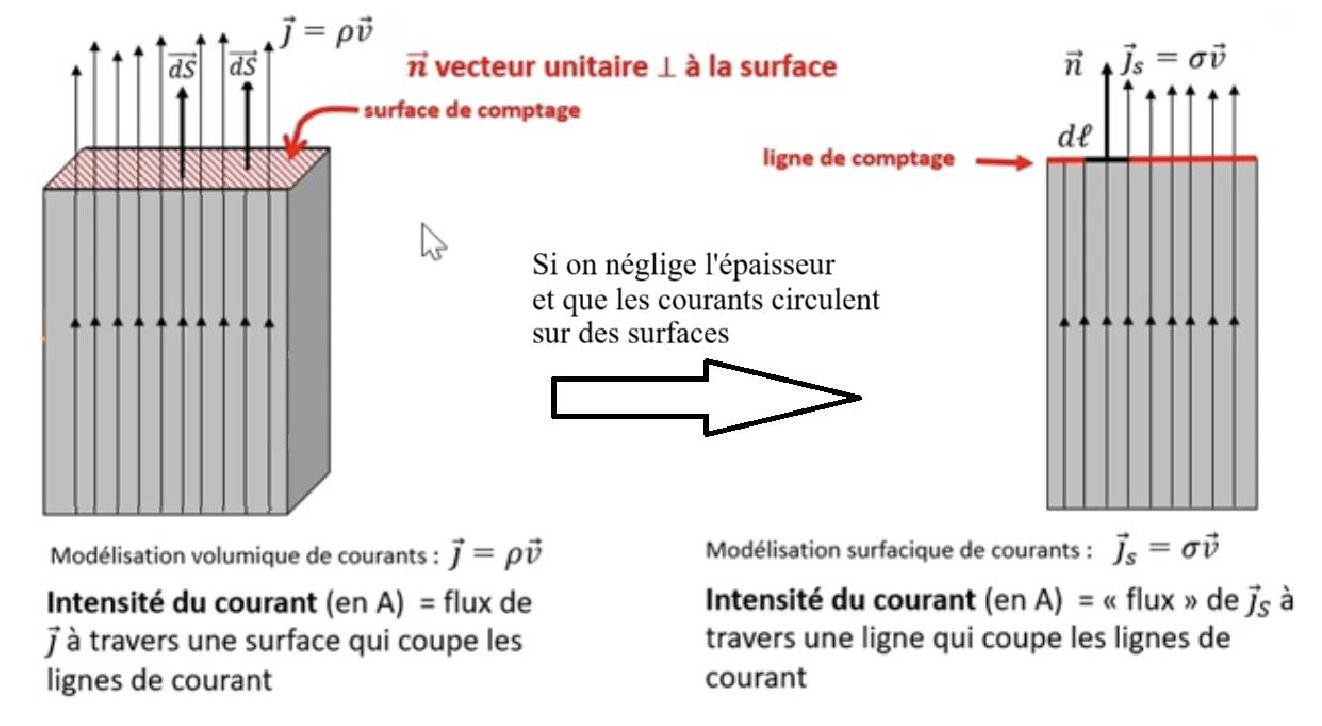
\includegraphics[width=0.8\textwidth]{./assets/Intensité du courant surfacique.png}
        \caption{Intensité du courant surfacique}
        \label{Intensité du courant surfacique}
      \end{figure}

      
\end{itemize}
\end{Prop}

\subsection{Distribution stationaire} % (fold)
\label{sub:Distribution stationaire}

Les distributions sont dites stationaires si elles sont indépendantes du temps : 

\begin{equation}
  \frac{\partial \rho}{\partial t} (M,t) = 0 ,\quad \frac{\partial \overrightarrow{j}}{\partial t} (M, t)= 0
\end{equation}
% subsection Distribution stationaire (end)
\subsection{Conservation de la charge}

\begin{Prop}{Equation locale de la conservation de charge}{}
  \[
    \mathrm{div} \overrightarrow{j}(M,t) + \frac{\partial \rho}{\partial t} (M,t) = 0
  \]
\end{Prop}

\begin{myproof}{}{}
  \begin{figure}[H] %h:当前位置, t:顶部, b:底部, p:浮动页
    \centering
    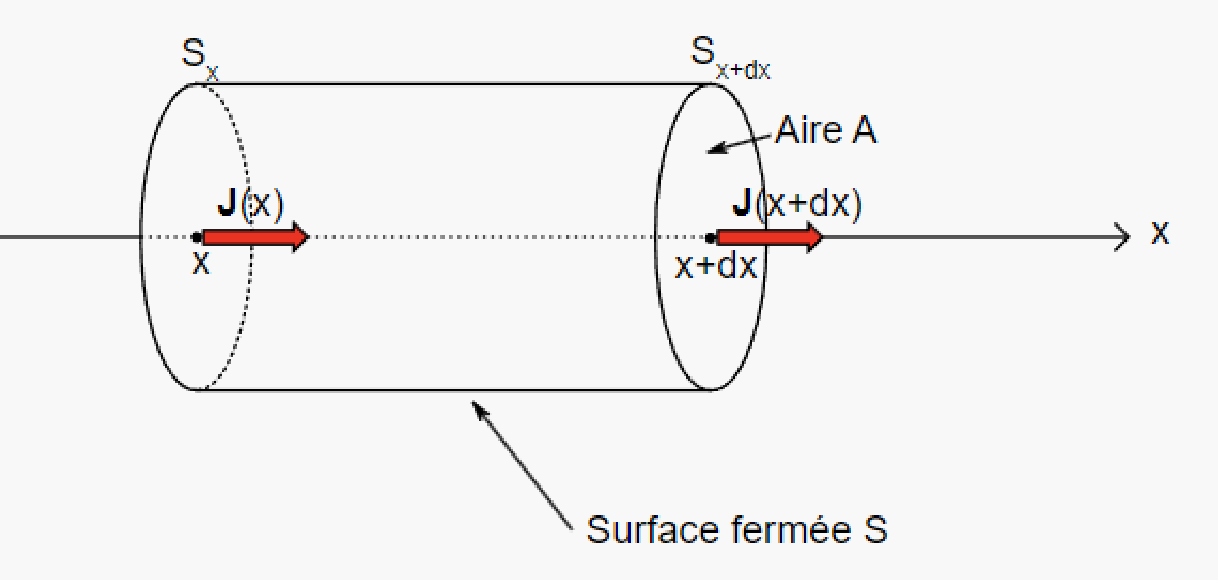
\includegraphics[width=0.5\textwidth]{./assets/Preuve - Conservation des charges.png}
    \caption{Preuve - Conservation des charges}
    \label{fig:Preuve - Conservation des charges}
  \end{figure}

  
\begin{itemize}

    \item À la date $t$, il y a une quantité de charge : $\mathrm{d}^2q(t) = \rho(x,t) \mathrm{d} \tau$, et à la date $t + \mathrm{d}t$, $\mathrm{d}^2q(t + \mathrm{d}t ) = \rho (x, t+ \mathrm{d}t) \mathrm{d}\tau$ dans le volume $\mathrm{d}\tau$.

    \item Bilan spatial :
      \begin{align*}
        \delta ^2 q &= \delta ^2 q _\text{entrant} - \delta ^2 q_\text{sortant} \\
                    &= \iint _{(S)} \overrightarrow{j}(x,t) . \overrightarrow{\mathrm{d}S} \mathrm{d}t  - \iint _{(S)} \overrightarrow{j}(x+ \mathrm{d}x,t) . \overrightarrow{\mathrm{d}S} \mathrm{d}t \\
                    &= [j(x,t) - j(x+ \mathrm{d}x)] S. \mathrm{d}t \\
                    &= - \mathrm{d}x. \frac{\partial j(x,t)}{\partial x}  S. \mathrm{d}t \\
      \end{align*}
      Donc, 
      \[
        - \mathrm{d}x . \frac{\partial j(x,t)}{\partial x} S \mathrm{d} t = \frac{\partial \rho(x,t)}{\partial t} \mathrm{d}t . \mathrm{d} \tau
      \]
      Finalement, 
      \[
        \frac{\partial j(x,t)}{\partial x}  + \frac{\partial \rho(x,t)}{\partial t}  = 0
      \]
\end{itemize}
\end{myproof}

\begin{myproof}{}{}
      Généralisation à (3D) : - Flux sortant = Changement de densité : 
      \begin{gather}
        \iiint _ V \frac{\partial \rho(M,t)}{\partial t}  \mathrm{d} \tau = \oiint _ \Sigma - \overrightarrow{j}(P,t) \overrightarrow{n} . \mathrm{d} S \\  
        \iiint _ V \left[ \frac{\partial \rho(M,t)}{\partial t}  + \mathrm{div} \overrightarrow{j}(M,t) \right] \mathrm{d} \tau = 0
      \end{gather}
\end{myproof}



\begin{Prop}{Conséquences en régime stationaire}{}

  \begin{itemize}

      \item Si $\rho$ indépendant du temps, alors $\mathrm{div} \overrightarrow{j} = 0$
      \item On en déduit que $\overrightarrow{j}$ est à flux \underline{conservatif}
      \item Le long d'un tube de champ, $I_1 = I_2$ 
      \item La loi des noeuds

  \end{itemize}

\end{Prop}


\subsection{Champs statiques} % (fold)
\label{sub:Champs statiques}

\begin{itemize}

    \item Soit une charge immobile $q_t$ placée en un point $M$. Plongée dans un champ $\overrightarrow{E}(M)$, cette charge subie une force $\overrightarrow{F} = q_t \overrightarrow{E}(M)$
    \item Soit une charge \underline{mobile} $q_t$ se déplaçant à la vitesse $\overrightarrow{v}$. Plongée dans un champ $\overrightarrow{B}(M)$, cette charge subie une force $\overrightarrow{F} = q_t \overrightarrow{v} \wedge\overrightarrow{B}(M)$

\end{itemize}
% subsection Champs statiques (end)


\newpage 
\section{Mathématique : Opérateurs} % (fold)
\label{sec:Mathématique : Opérateurs}

Voir le dossier \href{http://moodle.speit.sjtu.edu.cn/pluginfile.php/37446/mod_resource/content/1/De_Formulaire_analyse_vectorielle_P2021.pdf}{Formulaire d'analyse vectorielle}

\subsection{Relations entre opérateurs} % (fold)
\label{sub:Relations entre opérateurs}

\begin{gather}
  \mathrm{div} (\overrightarrow{\mathrm{rot}} \overrightarrow{X}) = 0 \\ 
  \mathrm{div} ( \overrightarrow{\mathrm{grad}} X) = \Delta X \\ 
  \overrightarrow{\mathrm{rot}} ( \overrightarrow{\mathrm{rot}} \overrightarrow{X}) = \overrightarrow{\mathrm{grad}}(\mathrm{div} \overrightarrow{X}) - \Delta \overrightarrow{X}
\end{gather}
% subsection Relations entre opérateurs (end)

\subsection{L'opérateur nabla} % (fold)
\label{sub:L'opérateur nabla}

\begin{gather}
  \overrightarrow{\mathrm{grad}} A = \overrightarrow{\nabla} A \\ 
  \mathrm{div} \overrightarrow{X} = \overrightarrow{\nabla}. \overrightarrow{X} \\ 
  \overrightarrow{\mathrm{rot}} \overrightarrow{X} = \overrightarrow{\nabla} \wedge \overrightarrow{X}\\ 
  \Delta A = \overrightarrow{\nabla} . \overrightarrow{\nabla} A
\end{gather}
% subsection L'opérateur nabla (end)
% section Mathématique : Opérateurs (end)

\newpage
\section{Postulats fondamentaux de l'électromagnétisme} % (fold)
\label{sec:Postulats fondamentaux de l'électromagnétisme}

\subsection{Force de Lorentz} % (fold)
\label{sub:Force de Lorentz}
\begin{equation}
  \overrightarrow{F} = q_t ( \overrightarrow{E} (M,t) + \overrightarrow{v} \wedge \overrightarrow{B}(M,t))
\end{equation}
% subsection Force de Lorentz (end)

\subsection{Équations de Maxwell} % (fold)
\label{sub:Équations de Maxwell}

\begin{Theorem}{Equations de Maxwell}{}

  Le champ électromagnétique et les densité de charge et de courant vérifient localement 4 équations : 
\begin{gather}
  \text{Équation de Maxwell-Gauss} \quad \mathrm{div} \overrightarrow{E} (M,t) = \frac{\rho(M,t)}{\varepsilon_0}  \\ 
\text{Équation de conservation du flux magnétique} \quad  \mathrm{div} \overrightarrow{B} (M,t) = 0 \\ 
\text{Équation de Maxwell-Faraday} \quad   \overrightarrow{\mathrm{rot}} \overrightarrow{E}(M,t ) = - \frac{\partial \overrightarrow{B}(M,t)}{\partial t}  \\ 
\text{Équation de Maxwell-Ampère} \quad \overrightarrow{\mathrm{rot}} \overrightarrow{B}(M,t ) = \mu_0 \left(\overrightarrow{j}(M) + \varepsilon_0 \frac{\partial \overrightarrow{E}(M,t)}{\partial t} \right)
\end{gather}
\end{Theorem}


\subsubsection{Cas statique} % (fold)
\label{sec:Cas statique}

% subsubsection Cas statique (end)
\begin{Prop}{Equations de Maxwell statique}{}
\begin{gather}
  \mathrm{div} \overrightarrow{E} (M) = \frac{\rho(M)}{\varepsilon_0}  \\ 
  \mathrm{div} \overrightarrow{B} (M) = 0 \\ 
  \overrightarrow{\mathrm{rot}} \overrightarrow{E}(M) = \overrightarrow{0} \\ 
  \overrightarrow{\mathrm{rot}} \overrightarrow{B}(M) = \mu_0 \overrightarrow{j}(M)
\end{gather}
\end{Prop}
\subsubsection{Remarques} % (fold)
\label{sec:Remarques}

% subsubsection Remarques (end)
\begin{Definition}[colbacktitle=red!75!black]{Vecteur densité de courant de déplacement}{}
\begin{equation}
  \overrightarrow{j_D}(M,t) = \varepsilon_0 \frac{\partial \overrightarrow{E}(M,t)}{\partial t} 
\end{equation}
\end{Definition}


\subsubsection{Linéarité} % (fold)
\label{sec:Linéarité}

% subsubsection Linéarité (end)

\begin{Prop}{Principe de superposition}{}
Les équations de Maxwell sont linéaires. Les solutions vérifient le principe de superposition. 
\end{Prop}

\subsubsection{Couplage} % (fold)
\label{sec:Couplage}

% subsubsection Couplage (end)
\begin{Prop}{Couplage}{}
Les équations de Maxwell donne deux types de couplages :
\begin{itemize}

    \item Deux champs, électronique et magnétique
    \item Deux champs de distribution, courant et charges

\end{itemize}

Les champs $\{\overrightarrow{j}(M,t), \; \rho(M,t)\}$ sont conjointment sources des champs électroniques et magnétiques.

\end{Prop}

\subsubsection{Application : Vérification de la conservation de la charge} % (fold)

% subsubsection Application (end)
\begin{Prop}{Conservation de la charge}{}
  \begin{equation}
    \mathrm{div} \overrightarrow{j} + \frac{\partial \rho}{\partial t}  = 0
  \end{equation}

\end{Prop}
\begin{myproof}{}{} Utilise $\mathrm{div}(MA)$ et $\mathrm{div} \overrightarrow{E}$
\begin{gather}
 \mathrm{div} (\overrightarrow{\mathrm{rot}}\overrightarrow{B}) = \mu_0 \mathrm{div} \left( \overrightarrow{j} + \varepsilon_0 \frac{\partial \overrightarrow{E}}{\partial t}  \right) \\ 
  0 = \mathrm{div} \overrightarrow{j} + \varepsilon_0 \frac{\partial }{\partial t} (\mathrm{div} \overrightarrow{E} )
\end{gather}
\end{myproof}

\subsection{Loi d'Ohm} % (fold)
\label{sub:Loi d'Ohm}

Présentera dans la partie \ref{sub:Loi d'Ohm locale} :

\begin{Theorem}{Loi d'Ohm}{}
Pour un conducteur électrique, 
\begin{equation}
  \overrightarrow{j}(M,t) = \gamma \overrightarrow{E}(M,t)
\end{equation}
\end{Theorem}
% subsection Loi d'Ohm (end)

\newpage
\section{Symétries du champ électromagnétique} % (fold)
\label{sec:Symétries du champ électromagnétique}

Considérons une source constituée de charge et de courant de distributions $\{\rho(P,t), \overrightarrow{j}(P,t)\}$, 
\begin{itemize}

    \item Les plans de \underline{symétrie} des sources sont les plans de \underline{symétrie} du champ $\overrightarrow{E}$ et les plans d'\underline{anti-symétrie} du champ $\overrightarrow{B}$.

      \begin{figure}[H] %h:当前位置, t:顶部, b:底部, p:浮动页
        \centering
        \includegraphics[width=0.5\textwidth]{./assets/Distribution symétrique.png}
        \caption{Distribution symétrique}
      \end{figure}



      
    \item Les plans de \underline{anti-symétrie} des sources sont les plans de \underline{anti-symétrie} du champ $\overrightarrow{E}$ et les plans d'\underline{symétrie} du champ $\overrightarrow{B}$.

\begin{figure}[H] %h:当前位置, t:顶部, b:底部, p:浮动页
  \centering
  \includegraphics[width=0.5\textwidth]{./assets/Distribution anti-symétrique.png}
  \caption{Distribution anti-symétrique}
\end{figure}

\end{itemize}
% section Symétries du champ électromagnétique (end)
\section{Champ électromagnétique dans le vide} % (fold)
\label{sec:Champ électromagnétique dans le vide}

\subsection{Opérateur Laplacien vectoriel} % (fold)
\label{sub:Operateur Laplacien vectoriel}

% subsection Operateur Laplacien vectoriel (end)
\begin{Definition}[colbacktitle=red!75!black]{Opérateur Laplacien vectoriel}{}
\begin{equation}
  \Delta \overrightarrow{A} = \overrightarrow{\mathrm{grad}} ( \mathrm{div} \overrightarrow{A}) - \overrightarrow{\mathrm{rot}} (\overrightarrow{\mathrm{rot}} \overrightarrow{A})
\end{equation}
\end{Definition}

\begin{Example}{Coordonnées cartésiennes}{}
\begin{equation}
  \Delta \overrightarrow{A} = \begin{pmatrix}
    \Delta A_x \\
    \Delta A_y \\
    \Delta A_z 
  \end{pmatrix} = \begin{pmatrix}
  \frac{\partial ^{2}A_x}{\partial x ^{(2)}} + \frac{\partial ^{2} A_{\color{red} x}}{\partial y^{2}} + \frac{\partial ^{2} A_{\color{red} x}}{\partial z ^{(2)}} \\ 
  \frac{\partial ^{2}A_y}{\partial x ^{(2)}} + \frac{\partial ^{2} A_{\color{red} y}}{\partial y^{2}} + \frac{\partial ^{2} A_{\color{red} y}}{\partial z ^{(2)}} \\ 
  \frac{\partial ^{2}A_z}{\partial x ^{(2)}} + \frac{\partial ^{2} A_{\color{red} z}}{\partial y^{2}} + \frac{\partial ^{2} A_{\color{red} z}}{\partial z ^{(2)}}  
  \end{pmatrix}
\end{equation}
\end{Example}

\subsection{Équations de Maxwell dans le vide} % (fold)

% subsection  (end)
\begin{Prop}{Champ Électromagnétique dans le vide}{}
Dans le vide,
\begin{itemize}
    \item Equation de Maxwell-Gauss (M.G.)
        \[
        \mathrm{div} \overrightarrow{E} (M,t) = 0
        \]
    \item Equation de Mawell-Flux (M.$\varphi$.)
        \[
        \mathrm{div} \overrightarrow{B} (M,t) = 0
        \]
    \item Equation de Maxwell-Faraday (M.F.)
        \[
        \overrightarrow{\mathrm{rot}}\overrightarrow{E} (M,t) = - \frac{\partial \overrightarrow{B} (M,t)}{\partial t}  
        \]
    \item Equation de Maxwell-Ampère (M.A.)
        \[
        \overrightarrow{\mathrm{rot} }  \overrightarrow{B} (M,t) = \varepsilon_0\mu_0 \frac{\partial \overrightarrow{E} (M,t)}{\partial t} 
        \]
\end{itemize}
\end{Prop}

\begin{Prop}{Équations de d'Alembert}{}
Les champs $\overrightarrow{E} (M,t)$ et $\overrightarrow{B} (M,t)$ peuvent être découplés, on obtient alors les équations de d'Alembert :
\begin{align*}
    \Delta \overrightarrow{E}  - \frac{1}{c^{2}} \frac{\partial ^{2}\overrightarrow{E} }{\partial t^{2}}  &= \overrightarrow{0} \\
    \Delta \overrightarrow{B}  - \frac{1}{c^{2}} \frac{\partial ^{2}\overrightarrow{B} }{\partial t^{2}}  &= \overrightarrow{0}
\end{align*}
\end{Prop}

\begin{myproof} Rappel que : $\overrightarrow{\mathrm{rot}}\overrightarrow{\mathrm{rot}}\overrightarrow{A} = \overrightarrow{\mathrm{grad}}\mathrm{div}\overrightarrow{A} - \Delta \overrightarrow{A}$
\begin{gather*}
    \overrightarrow{\mathrm{rot} } (\overrightarrow{\mathrm{rot} } \overrightarrow{E}) = \overrightarrow{\mathrm{rot} } \left( - \frac{\partial \overrightarrow{B} }{\partial t}  \right)  \\
\overrightarrow{\mathrm{grad} } \mathrm{div} \overrightarrow{E}  - \Delta \overrightarrow{E}  = - \frac{\partial }{\partial t} (\overrightarrow{\mathrm{rot} } \overrightarrow{B} )\\
-\Delta \overrightarrow{E}  = - \frac{\partial }{\partial t} \left( \varepsilon_0 \mu_0 \frac{\partial \overrightarrow{E} }{\partial t}  \right)  \\
    \Delta \overrightarrow{E}  - \frac{1}{c^{2}} \frac{\partial ^{2}\overrightarrow{E} }{\partial t^{2}}  = \overrightarrow{0}
\end{gather*}
On note $c^{2} = 1 / (\varepsilon_0 \mu_0)$, de même façon, on calcule le rotation de l'équation de (M.A)
\end{myproof}


\newpage
\section{Formulation intégrale de l'électromagnétisme} % (fold)

\subsection{Outil mathématique} % (fold)
\label{sub:Outil mathématique}

% subsection Outil mathématique (end)
\label{sec:Formulation intégrale de l'électromagnétisme}
\begin{Theorem}{Théorème de Green-Ostrogradski}{}
\begin{equation}
  \oiint _{(S)} \overrightarrow{A}. \overrightarrow{\mathrm{d}S _{ext}} = \iiint _{(V)} \mathrm{div} \overrightarrow{A} \mathrm{d} \tau
\end{equation}

Le flux d'un champ vectoriel $\overrightarrow{A}$ sortant d'une surface fermée $(S)$ est égal à l'intégrale de sa divergence étendue au volume $(V)$ délimité par $(S)$
\end{Theorem}

\begin{Theorem}{Théorème de Stokes}{}
\begin{equation}
  \oint _{(C)} \overrightarrow{A}. \overrightarrow{\mathrm{d}l} = \iint\overrightarrow{\mathrm{rot}} \overrightarrow{A}. \overrightarrow{\mathrm{d}S}
\end{equation}

La circulation du champ vectoriel $\overrightarrow{A}$ est égale au flux du rotationnel de $\overrightarrow{A}$ à travers toute surface $(S_c)$ s'appuyant sur un contour fermé \textbf{oritenté}.
\end{Theorem}



\subsection{Théorème de Gauss} % (fold)
\label{sub:Théorème de Gauss}
\begin{Theorem}{Théorème de Gauss}{}
\begin{gather}
  (MG) \quad \mathrm{div} \overrightarrow{E} = \frac{\rho}{\varepsilon_0}  \\
  (\text{Green-Ostrogradski}) \quad \oiint \overrightarrow{E} . \overrightarrow{\mathrm{d} S _{ext}} = \iiint \mathrm{div} \overrightarrow{E} \mathrm{d} \tau = \iiint \frac{\rho}{ \varepsilon_0} d\tau \\
  \boxed{\oiint \overrightarrow{E} . \overrightarrow{\mathrm{d} S _{ext}} = \frac{ Q _{int}
  }{\varepsilon_0} }
\end{gather}
\end{Theorem}

\subsubsection{Cas du vide} % (fold)
\label{sec:Cas du vide}
\begin{equation}
  Q _{int}  (t) = 0 \implies \oiint \overrightarrow{E}(M,t) . \overrightarrow{n _{ext, M}} \mathrm{d} S = 0
\end{equation}

Le champ électrique dans le vide est donc à \underline{flux conservatif} ($\mathrm{div} \overrightarrow{E} = 0$)

\begin{Example}{}{}
Une sphère chargée de rayon $R$, placée dans un conducteur ohmique de conductivité $\gamma$. La charge totale de la sphère évolue avec le temps. 
\end{Example}

\begin{myproof}{}{}
    \begin{gather}
      E(R,t) \times 4 \pi R ^{2}  = \frac{Q(t)}{\varepsilon_0}  \\ 
      \frac{\mathrm{d}Q (t)}{\mathrm{d} t}  = - J(R,t) \times 4 \pi R ^{2} \\ 
      J(R, t) = \gamma E(R, t) \\ 
      \frac{\mathrm{d}Q(t)}{\mathrm{d}t}  + \frac{\gamma}{\varepsilon_0}  Q(t) = 0 \implies Q(t) = Q_0 \exp \left( - \frac{t}{\tau}  \right)
    \end{gather}
\end{myproof}




\subsection{Conservation du flux magnétique} % (fold)
\label{sub:Conservation du flux magnétique}

\begin{Theorem}{Conservation du flux magnétique}{}

  \begin{gather}
    (M \Phi) \quad \mathrm{div} \overrightarrow{B} = 0 \\ 
  (\text{Green-Ostrogradski}) \quad \oiint \overrightarrow{B} . \mathrm{d} S \overrightarrow{S} _{ext} = \iiint \mathrm{div} \overrightarrow{B} . \mathrm{d} \tau = 0
  \end{gather}

Donc, \underline{le flux de $\overrightarrow{B}$ à travers une surface fermée est nul}.
\end{Theorem}



\subsubsection{Conséquence} % (fold)
\label{sec:Conséquence}
\begin{itemize}

    \item \textbf{Tube de champ $\overrightarrow{B}$} : Le flux de $\overrightarrow{B}$ à travers une section de tube de champ est indépendant de cette section. (= champ magnéstostatique) 

    \item Notion de \textbf{flux à travers un contour} : Le flux de $\overrightarrow{B}$ à travers une surface \underline{s'appuyant sur un contour} ne dépend que du contour, et pas de la surface particulière choisie. 
      \begin{equation}
        \iint \overrightarrow{B}. \overrightarrow{n_1} \mathrm{d} S = \iint \overrightarrow{B} . \overrightarrow{n_2} \mathrm{d}S
      \end{equation}

\end{itemize}
% subsubsection Conséquence (end)
% subsect:ion Conservation du flux magnétique (end)
% subsubsection Cas du vide (end)

% subsection Théorème de Gauss (end)

\subsection{Loi de Faraday} % (fold)
\label{sub:Loi de Faraday}


\begin{Theorem}{Loi de Faraday}{}
  Notons $\Phi _{\overrightarrow{B}/(C)}$ le flux du champ $\overrightarrow{B}$ à travers la surface $S_C$ donc à travers le contour $C$ : 
\begin{gather}
  \overrightarrow{\mathrm{rot}} \overrightarrow{E} (M,t) = - \frac{\partial \overrightarrow{B}}{\partial t} (M,t) \\ 
  \oint _{{(c)}} \overrightarrow{E} (M,t) . \overrightarrow{\mathrm{d}l_M} = \iint _{(S_c)} - \frac{\partial  \overrightarrow{B}}{\partial t} (M,t) . \overrightarrow{n_M}. \mathrm{d}S_M = - \frac{\mathrm{d}}{\mathrm{d}t}  \iint _{(S_C)} \overrightarrow{B}(M,t) . \overrightarrow{n_M}. \mathrm{d} S_M \\ 
  \boxed{\oint _{(C)} \overrightarrow{E}(M,t). \overrightarrow{\mathrm{d}l_M} = - \frac{\mathrm{d} \Phi _{\overrightarrow{B}/(C)}}{\mathrm{d}t} (t)}
\end{gather}
\end{Theorem}

\subsubsection{Cas stationaire} % (fold)
\label{sec:Cas stationaire}
\begin{equation}
  - \frac{\mathrm{d} \Phi _{\overrightarrow{B}/(C)}}{\mathrm{d}t} (t) = 0 \implies \oint _{(C)}  \overrightarrow{E}(M,t). \overrightarrow{\mathrm{d} l_M} = 0
\end{equation}

Le champ \underline{électrostatique} est à circulation conservative. Donc, c'est impossible d'avoir des lignes de champ électrique fermée. 

MAIS, en régime dépendant du temps, ils peuvent être fermées !!
% subsubsection Cas stationaire (end)

\subsection{Théorème d'Ampère} % (fold)
\label{sub:Théorème d'Ampère}
\begin{Theorem}{Théorème d'Ampère}{}
Théorème d'Ampère généralisé :
\begin{gather}
  (MA) \quad \overrightarrow{\mathrm{rot}} \overrightarrow{B} = \mu_0 \overrightarrow{j} + \varepsilon_0 \mu_0 \frac{\partial \overrightarrow{E}}{\partial t}  \\ 
  (\text{Théorème de Stokes}) \quad \oint _{(C)} \overrightarrow{B} (M,t) . \overrightarrow{\mathrm{d}l_M} = \mu_0 \iint _{(S_c)} \overrightarrow{j} (M,t) . \overrightarrow{n_M} \mathrm{d} S_M + \mu_0 \iint _{(S_c)}  \varepsilon_0 \frac{\partial  \overrightarrow{E}(M,t)}{\partial t} . \overrightarrow{n_M} \mathrm{d} S_M \\ 
  \boxed{\oint _{(C)} \overrightarrow{B} (M,t) . \overrightarrow{\mathrm{d}l_M} = \mu_0 \iint _{(S_c)} \overrightarrow{j} (M,t) . \overrightarrow{n_M} \mathrm{d} S_M + \mu_0  \iint _{(S_c)} \varepsilon_0 \frac{\partial  \overrightarrow{E}(M,t)}{\partial t} . \overrightarrow{n_M} \mathrm{d} S_M }
\end{gather} 
\end{Theorem}

\subsubsection{Intensité du courant de déplacement} % (fold)
\label{sec:Intensité du courant de déplacement}
\begin{equation}
    \boxed{\oint _{(C)} \overrightarrow{B} (M,t) . \overrightarrow{\mathrm{d}l_M} = \mu_0 (I _{\text{enlacé}}+ I _{D})}
\end{equation}

Notant l'\textbf{intensité du courant de déplacement} :
\begin{equation}
  I _{D, (S_c)} = \varepsilon_0 \frac{\mathrm{d}}{\mathrm{d}t}  \iint _{(S_C)} \overrightarrow{E} (M,t) \overrightarrow{n}_M \mathrm{d} S_M
\end{equation}
% subsubsection Intensité du courant de déplacement (end)
\subsection{Cas des distributions surfaciques} % (fold)

Remarque : 

\begin{itemize}

    \item 
Dans un distribution \underline{volumique}, $\overrightarrow{E}$ et $\overrightarrow{B}$ sont continues en tout point.

\item Le potentiel est TOUJOURS continue.

\end{itemize}

\subsubsection{Champ électrique} % (fold)
\label{sec:Champ électrique}

% subsubsection Champ électrique (end)
Considérons une distribution de charges où les charges sont localisées sur le plan infini $z=0$ avec une densité de charge uniform $\sigma$. À l'aide du théorème de Gauss, le champ électrostatique est : 
\begin{equation}
  \overrightarrow{E} (z) = \frac{\sigma}{2\epsilon_0}  \overrightarrow{e_z} (z>0),
  \quad\overrightarrow{E} (z) = -\frac{\sigma}{2\epsilon_0}  \overrightarrow{e_z} (z<0)
\end{equation}

Le champ électrique est donc discontinue en $z=0$, avec la discontinuité 
\begin{equation}
  \overrightarrow{E}(z= 0 ^{+}) - \overrightarrow{E} ( z= 0 ^{-}) = \frac{\sigma}{\varepsilon_0}  \overrightarrow{e_z}
\end{equation}

\begin{Prop}[colbacktitle=red!75!black]{Relation de passage pour le champ électrique}{}
  Cas général :
\begin{equation}
  \overrightarrow{E}(M ^{+}, t) - \overrightarrow{E}(M ^{-},t) = \frac{\sigma(M,t)}{\varepsilon_0}  \overrightarrow{n_M}
\end{equation}
\end{Prop}

\begin{itemize}

    \item Continuité de la composante tangentielle du champ électrique 
\begin{gather}
(\overrightarrow{E_2} - \overrightarrow{E_1}) . \overrightarrow{t _{1 \to 2}}  = \frac{\sigma}{\varepsilon_0}  \overrightarrow{n _{1 \to 2}} . \overrightarrow{t _{1 \to 2}} \\ 
E _{2T} - E_{1T} = 0 \implies E _{2T} = E _{1T}
\end{gather}
    \item Discontinuité de la composante normale du champ électrique

\end{itemize}


\subsubsection{Champ magnétique} % (fold)
\label{sec:Champ magnétique}

\begin{Prop}{Relation de passage pour le champe magnétique}{}
Cas général :
\begin{equation}
  \overrightarrow{B} (M ^{+}, t) - \overrightarrow{B}( M ^{-}, t) = \mu_0 \overrightarrow{j_S}(M,t) \wedge \overrightarrow{n_M}
\end{equation}

\end{Prop}
\begin{itemize}




    \item Discontinuité de la somposante tangentielle du champ magnétique 

    \item Continuité de la composante normale du champ magnétique

\end{itemize}
% subsubsection Champ magnétique (end)


\newpage
\section{Potentiel scalaire et potentiel vecteur, Approximation des Régimes Quasi Stationaires}
\subsection{Définitions} % (fold)
\label{sub:Définitions}

% subsection Définitions (end)

\begin{Definition}[colbacktitle=red!75!black]{Potentiel vecteur et Potentiel scalaire}{}
  \textbf{Potentiel vecteur} : 
\begin{gather}
  (M\varphi) \quad \mathrm{div} \overrightarrow{B} = 0 \implies
  \exists \overrightarrow{A}(M,t), \;\boxed{\overrightarrow{B}(M,t) = \overrightarrow{\mathrm{rot}} \overrightarrow{A} (M,t)}, \quad \mathrm{div} ( \overrightarrow{\mathrm{rot}}\overrightarrow{A}) = \overrightarrow{\nabla}. \overrightarrow{\nabla } \wedge \overrightarrow{A}= 0  
\end{gather}

\textbf{Potentiel scalaire} : en injectant dans l'équation $(MF)$ :
  \begin{gather}
  \overrightarrow{\mathrm{rot}} \overrightarrow{E} = - \frac{\partial }{\partial t} ( \overrightarrow{\mathrm{rot}} \overrightarrow{A}) = - \overrightarrow{\mathrm{rot}}( \frac{\partial \overrightarrow{A}}{\partial t} ) \\ 
  \overrightarrow{\mathrm{rot}} \left( \overrightarrow{E}(M, t) + \frac{\partial \overrightarrow{A}}{\partial t} (M,t) \right) = \overrightarrow{0} \\ 
  \exists V(M,t), \;\boxed{\overrightarrow{E}(M,t) = - \frac{\partial \overrightarrow{A}}{\partial t} (M,t) - \overrightarrow{\mathrm{grad}} V(M,t)}
  \end{gather}
\end{Definition}

\subsection{Indétermination} % (fold)
\label{sec:Indétermination}

% subsubsection Indétermination (end)
Soient deux couples de potentiels $\{\overrightarrow{A},V\}$ et $\{\overrightarrow{A'}, V'\}$ associé à un champ électromagnétique.

\begin{gather}
  \overrightarrow{B}(M,t) = \overrightarrow{\mathrm{rot}} \overrightarrow{A } = \overrightarrow{\mathrm{rot}}\overrightarrow{A} \implies \overrightarrow{\mathrm{rot}}(A - A') = \overrightarrow{0}
\end{gather}

Donc $(\overrightarrow{A} - \overrightarrow{A'})$ est à circulation conservative. Il existe un champ scalaire $g(M,t)$ tel que :
\begin{equation}
  \boxed{  \overrightarrow{A} - \overrightarrow{A'} = - \overrightarrow{\mathrm{grad}}g}
\end{equation}

Ensuite, 

\begin{gather}
    - \frac{\partial \overrightarrow{A}}{\partial t}  - \overrightarrow{\mathrm{grad}}V = - \frac{\partial \overrightarrow{A'}}{\partial t}  - \overrightarrow{\mathrm{grad}}V' \\ 
    \overrightarrow{\mathrm{grad}} ( V - V') = - \frac{\partial }{\partial t} (\overrightarrow{A'} - \overrightarrow{A}) = - \frac{\partial }{\partial t} (- \overrightarrow{\mathrm{grad}} g ) \\ 
    \boxed{V - V' = \frac{\partial g}{\partial t} }
\end{gather}

Conclusion : 
\begin{equation}
  \overrightarrow{A'}(M,t) = \overrightarrow{A}(M,t) +  \overrightarrow{\mathrm{grad}} g (M,t) \quad \text{ et } \quad V'(M,t) = V (M, t) - \frac{\partial g}{\partial t} (M,t)
\end{equation}

\textbf{Transformation de jauge} : transformation qui fait passe d'un couple de potentiel à un autre.
\subsection{Jauge de Coulomb} % (fold)
\label{sec:Jauge de Coulomb}
En régime statique ou quasi-statique, il est commode de shoisir un potentiel vecteur 
\begin{itemize}

    \item indépendant du temps 
    \item La condition : \textbf{Jauge de Coulomb} : $\boxed{\mathrm{div}\overrightarrow{A}(M,t)= 0}$

\end{itemize}

\subsection{Jauge de Lorentz} % (fold)
\label{sec:Jauge de Lorentz}
En régime dépendant du temps, il est plus intérssant de fixer la condition, appelée \textbf{Jauge de Lorentz} : 
\begin{equation}
  \mathrm{div} \overrightarrow{A}(M,t) + \varepsilon_0 \mu_0 \frac{\partial V}{\partial t} (M,t) = 0
\end{equation}

\subsection{Equations de Poisson retardées} % (fold)
\label{sec:Equations de Poisson retardées}

Dans le cas de la juage de Lorentz, on peut découpler $V$ et $\overrightarrow{A}$

\begin{Prop}{Equations de Poisson retardées}{}
  \begin{itemize}

      \item \textbf{Potentiel scalaire} :
        \begin{equation}
          \Delta V(M,t) - \frac{1}{c ^{2}}  \frac{\partial ^{2}V(M,t)}{\partial t ^{2}}  = - \frac{\rho(M,t)}{\varepsilon_0} 
        \end{equation}
      \item \textbf{Potentiel vecteur} :
        \begin{equation}
          \Delta \overrightarrow{A}(M,t) - \frac{1}{c ^{2}}  \frac{\partial ^{2} \overrightarrow{A}(M,t)}{\partial t ^{2}}  = - \mu_0 \overrightarrow{j}(M,t)
        \end{equation}


  \end{itemize}
\end{Prop}

\begin{myproof}{}{} Respectivement, 
\begin{gather}
  \mathrm{div} \overrightarrow{E} = \mathrm{div} \left( - \frac{\partial \overrightarrow{A}}{\partial t} - \overrightarrow{\mathrm{grad}}V \right) = \varepsilon_0 \mu_0 \frac{\partial  ^{2}V}{\partial t ^{2}}  - \Delta V = \frac{\rho}{\varepsilon_0}  \\ 
  \Delta \overrightarrow{A} = \overrightarrow{\mathrm{grad}}(\mathrm{div} \overrightarrow{A}) - \overrightarrow{\mathrm{rot}}\overrightarrow{\mathrm{rot}}\overrightarrow{A} = \overrightarrow{\mathrm{grad}} \left( - \varepsilon_0 \mu_0 \frac{\partial V}{\partial t} (M,t) \right) - \overrightarrow{\mathrm{rot}}\overrightarrow{B} \\ 
\overrightarrow{\mathrm{rot}} \overrightarrow{B} = \mu_0 (\overrightarrow{j} + \overrightarrow{j_D}) = \mu_0 \overrightarrow{j} + \mu_0 \varepsilon_0 \frac{\partial }{\partial t} \left( - \frac{\partial \overrightarrow{A}}{\partial t}  - \overrightarrow{\mathrm{grad}}V \right)
\end{gather}


\end{myproof}



\subsection{Solutions des potentiels retardés} % (fold)
\label{sub:Solutions des potentiels retardés}

\begin{equation}
  V(M,t) = \iiint _{(D)} \frac{1}{4 \pi \varepsilon_0} \frac{\rho(P, t - PM/c)}{PM}  \mathrm{d} \tau_P, \quad 
  \overrightarrow{A}(M,t) = \iiint _{(D)} \frac{\mu_0}{4 \pi} \frac{\overrightarrow{j}(P, t - PM/c)}{PM}  \mathrm{d} \tau_P
\end{equation}

Dans le cas de distributions statiques, nous retrouvons les expressions rencontrées en électrostatique et magnétostatique.
% subsection Solutions des potentiels retardés (end)

\begin{tcolorbox}
Notation : 

    ARQS = \textbf{Approximation des Régimes Quasi Stationnaires}
\end{tcolorbox}

\subsection{Valabilité d'ARQS} % (fold)

Tout changement des sources en $P$ est immédiatement perceptible en tout point $M$ : 
\begin{equation}
  \rho(P, t - PM/c) \approxeq \rho(P,t), \; \overrightarrow{j}(P, t - PM/c) \approxeq \overrightarrow{j}(P,t)
\end{equation}

ARQS valable si : 
\begin{equation}
  PM \ll \lambda, \; \frac{PM}{c}  \ll \tau
\end{equation}

\subsection{Champ magnétique ARQS} % (fold)
\label{sub:Champ magnétique}

Le champ magnétique sera donné par la même relation que l'expression du champ magnétostatique du même circuit.

\subsection{Champ électrique ARQS} % (fold)

La champ électrique n'est plus égal à celle du champ électrostatique : 
\begin{equation}
  \overrightarrow{E}(M,t) = \overrightarrow{E} _{QS}(t) - \frac{\partial \overrightarrow{A}}{\partial t} (M,t)
\end{equation}

